\documentclass[12pt]{article}
\usepackage{amsfonts, epsfig}
\usepackage[authoryear]{natbib}
\usepackage{graphicx}
\usepackage{fancyhdr}
\pagestyle{fancy}
\lfoot{\texttt{comsm0021.github.io}}
\lhead{Neural Information Processing - 3\_infomax - Conor}
\rhead{\thepage}
\cfoot{}
\begin{document}

\section*{Infomax}

The second topic we will consider is the Infomax algorithm. This is a
approach to unmixing mixed data proposed in \cite{BellSejnowski1995}
and gives an in-principle explanation for how the brain might perform
auditory source separation. In other words, it shows how source
separation might be performed and indicates some of the ingredients
that may be present in source separation in the brain.

The problem is as follows: imagine you are in a crowded room, in the
classic telling, at a cocktail party. Lots of people are talking, but
if you concentrate on one voice you can separate it from the overall
hub bub. We can experience the opposite effect when meditating or
sitting in thoughtful silence: we suddenly notice how loud distance
noises are, the noise of voices on the street, other people coughing
and clearing their throats, the sound of wind through nearby
trees. All these are sounds we automatically filter out when
listening. This process of picking out individual sources of sound
from a mixture of sounds is called auditory source separation, or, the
question of how to do this is called the cocktail party problem. In
fact, the problem is much more general than auditory source
separation; the same techniques should apply to any problem where we
can observe a mixed signal and would like the unmixed signal. In this
more general context the problem of source separation is called
independent component analysis.

As noted above, we are interested in the particularly neuronal
approach described in \cite{BellSejnowski1995}; however this isn't the
only approach to the problem and a different algorithm, fastICA
\citep{Hyvarinen1999}, is the most popular algorithm for source separation.

The problem can be phrased like this, given the sources
$\textbf{s}(t)$ where $\textbf{s}$ is a vector over multiple
sources. Now we do source separation with only two recordings, one for
each ear; here we are just going to consider the simpler problem of
source separation when there are as many recordings are as there are
sources, we also assume the mixing is linear and instantaneous, real
mixing of auditory signals in a room will only have these properties
approximately. However, given these assumption we have
\begin{equation} \mathbf{r}(t)=M\mathbf{s}(t) \end{equation} with $M$
a square mixing matrix. The goal is to find the unknown source signals
$\textbf{s}(t)$ from the known recordings $\textbf{r}(t)$. Although it
makes little difference, lets restrict ourselves to two sources, so
$\mathbf{s}$ and $\mathbf{r}$ are two-dimensional vectors and $M$ is a
two-by-two matrix.

We assume the two sources are independent,
$p_{S_1,S_2}=p_{S_1}p_{S_2}$; the point of source separation is to
unmix independent sources. Now, we want to find an unmixing matrix $W$ so that knowing
\begin{equation} {\bf x}(t)=W{\bf r}(t) \end{equation} is as good as
knowing the sources; precisely, since ${\bf x}=WM{\bf s}$ we want $WM$
to be a diagonal matrix multiplied by a permutation matrix, we do not
mind if unmixing changes the overall amplitude of the source, or if it
reorders the sources. In this two-to-two example, that means
\begin{equation} MW=\mbox{diag}\,(d_1,d_2) \end{equation} or
\begin{equation}
MW=\left(\begin{array}{cc}0&d_1\\d_2&0\end{array}\right)
\end{equation} where $d_1$ and $d_2$ are real numbers. Hence:
\begin{equation} {\bf s}\stackrel{\mbox{mixing}}{\longrightarrow}{\bf
r}=M{\bf s}\stackrel{\mbox{unmixing}}{\longrightarrow}{\bf x}=W{\bf r}
\end{equation}

One difficulty with looking at this problem is that it involves
continuous random variables, whereas the unit so far has
concentrated on the discrete case: $s_1(t)$ and $s_2(t)$ are continuous
variable. For this reason some of the results will just be quoted and
any exam questions will reflect the difficulty of this topic.

The main point with continuous random variables is that the
probability distribution is now a density, so 
\begin{equation}
Pr(a<x<b)=\int_a^b p_X(x) dx 
\end{equation} 
with 
\begin{equation}
\int_{-\infty}^{\infty} p_X(x)=1 dx
\end{equation} 
An important difference is demonstrated by the following formula: if
$Y=g(X)$ are two random variables related by an invertible function
$g$ 
\begin{equation} 
p_Y(y)=\frac{p_X(x=g^{-1}(y))}{|g'(x)|}
\end{equation}
In other words, the probability at $y$, $p_Y(y)$, is not just the
probability at the corresponding value of $x$, $p_X(g^{-1}(y))$, using
$x=g^{-1}(y)$, there is an additional scaling factor given by $g'(x)$.

To see roughly where this comes from, consider a simple scaling
$Y=\lambda X$, now, to preserve the probabilities
\begin{equation}
\int_{\lambda a}^{\lambda b} p_Y(y)dy=\int_{a}^b p_X(x)dx
\end{equation}
but if you do a change of variables $y=\lambda x$ on the left hand side this give
\begin{equation}
\int_a^b p_Y(\lambda x)\lambda dx=\int_{a}^b p_X(x)dx
\end{equation}
Thus, if $y=\lambda x$ then $g'(x)=\lambda$ and
\begin{equation}
p_Y(y)=\frac{p_x(x)}{\lambda}
\end{equation}

The information is defined in the same way as before
\begin{equation} 
H(X)=-\int  p(x)\log{p(x)} dx 
\end{equation} 
but it is no longer always positive. Furthermore, by substituting from
the formula above, you can see that
\begin{equation} 
H(\lambda X)=H(X)+\log{|\lambda|} 
\end{equation} 
and so the entropy has no maximum or minimum: a similar idea is the
maximization of entropy over distributions with the same variance and
this would rule out the scaling we see in this formula.

Now, the idea is to solve the problem by using the fact that $S_1$ and
$S_2$ are independent: we just need to find $W$ so that $X_1$ and
$X_2$ are also independent. One approach might be to decorrellate the
random variables:
\begin{equation}
C(X_1,X_2)=\langle(X_1-\langle X_1\rangle)(X_2-\langle X_2\rangle)\rangle_{(X_1,X_2)}
\end{equation}
where the expectation value for continuous random variables has the obvious definition
\begin{equation}
\langle g(X)\rangle =\int p_X(x)g(x) dx
\end{equation}
It is easy to check that the correlation vanishes if $X_1$ and $X_2$
are independent, however, the flaw in this approach is that the
converse is not true, it is possible to have zero correlation while
still having statistical dependence. To see this, imagine, for
convenience and without loss of generality, that $EX_1$ and $EX_2$ are
zero and that we have chosen $W$ so that the correlation matrix is the
identity:
\begin{equation}
C_{ab}=C(X_a,X_b)={\bf 1}
\end{equation}
then it is easy to see that rotations
\begin{equation}
\left(\begin{array}{c}X_1'\\X_2'\end{array}\right)=\left(\begin{array}{cc}\cos{\theta}&\sin{\theta}\\-\sin{\theta}&\cos{\theta}\end{array}\right)\left(\begin{array}{c}X_1\\X_2\end{array}\right)
\end{equation}
do not change the correlation matrix. Thus, the decorrelation
prescription has a rotational ambiguity and something more is
needed. That something, of course, is to require $I(X_1,X_2)=0$ since
this happens if and only if $X_1$ and $X_2$ are independent.

The problem is that $I(X_1,X_2)$ is difficult to calculate: the idea
behind infomax is to look at $H(X_1,X_2)$:
\begin{equation}
I(X_1,X_2)=H(X_1)+H(X_2)-H(X_1,X_2)
\end{equation}
The idea is that maximizing the joint entropy, $H(X_1,X_2)$ will give
a minimum of the mutual information, in other words, the variations in
the individual entropies $H(X_1)$ and $H(X_2)$ can be
ignored. However, as stated, this will not work because the entropy
can be increased by a trivial scaling, $X_a\rightarrow \lambda X_a$,
changes the joint entropy, $H(X_1,X_2)\rightarrow
H(X_1,X_2)+\log{|\lambda|}$ so $H(X_1,X_2)$ can be made arbitrarily
large by scaling, something that tells us nothing about mixing and
unmixing. Inspired by the behaviour of neurons, in
\cite{BellSejnowski1995} this is solved by adding a saturation
non-linearity:
\begin{eqnarray}
y_1&=&g(x_1+w_1)\cr
y_2&=&g(x_2+w_2)
\end{eqnarray}
where $w_1$ and $w_2$ are parameters and, for example,
\begin{equation}
g(u)=\frac{1}{1+e^{-u}}
\end{equation}
so $g:(-\infty,\infty)\rightarrow (0,1)$.
\begin{equation}
\epsfig{file=g.eps,width=4cm,angle=270}
\end{equation}

Now we have
\begin{equation}
{\bf s}\stackrel{\mbox{mixing}}{\longrightarrow}{\bf r}=M{\bf s}\stackrel{\mbox{unmixing}}{\longrightarrow}{\bf x}=W{\bf r}\stackrel{\mbox{non-linearity}}{\longrightarrow}{\bf y}:\,y_a=g(x_a+w_a)
\end{equation}
For later notational convenience, let write
\begin{equation}
y_a=g(x_a+w_a)=f(r_1,r_2;W,w_a)
\end{equation}
where $f$ is the function, parameterized by $W$ and $w_a$, mapping
from the recording to $y$. So reason the saturating non-linearity will
help is that with a non-linearity like this a large enough scaling
will reduce the entropy: consider $H(g(\lambda X))$ where $\lambda$ is
a constant. If $\lambda$ is very large it will spread $X$ out so that
it will take lots of very big positive or negative values; if $\lambda
x$ is a big positive number then $g(\lambda x)$ will be near to one,
conversely, if it is a large negative number, $g(\lambda x)$ will be
near to zero: a distribution that is often zero and often one is not
very entropic.

Before considering the source separation problem, lets look at the
effect of the non-linearity on its own: we consider the one-to-one
case
\begin{equation}
r\stackrel{\mbox{multiply}}{\longrightarrow}x=Wr\stackrel{\mbox{non-linearity}}{\longrightarrow}y=g(x+w)=f(r;w,W)
\end{equation}
where $W$ and $w$ are now both scalars and $r$, $x$ and $y$ are
outcomes for random variables $R$, $X$ and $Y$. We consider maximizing
the entropy $H(Y)$. What does this do; well, it maximizes the
information in $Y$ about $R$:
\begin{equation}
I(R;Y)=H(Y)-H(Y|R)
\end{equation}
but $H(Y|R)$ is constant since $R$ determines $Y$. In the discrete
case we are familiar with this would be easy to discuss, $H(Y|R)$
would be zero, in the continuous case it is not that simple, it is
actually minus infinity, but, the consequence is the same, it does not
depend on $W$ and $w$. To maximize $H(Y)$ we need to calculate its
derivative with respect to the parameters $W$ and $w$; this is a
feature of the algorithm, ultimately we need to calculate derivatives
and these are calculable and well defined, even if the quantity being
differentiated is not. In this case
\begin{equation}
H(Y)=-\int p(y)\log{p(y)} dy
\end{equation}
and this is estimated by
\begin{equation}
\tilde{H}(y)=-\log{p(y)}
\end{equation}
In other words, if $n$ values $y_i$ is drawn from $Y$ then 
\begin{equation}
\frac{1}{n}\sum_i\tilde{H}(y_i)\rightarrow H(Y)
\end{equation}
as $n$ gets large. 

Of course we do not have $p_Y(y)$ and it would be difficult to
estimate, but, it turns out we do not need it to get the derivative of
$\tilde{H(y)}$. We have seen already that since $y=f(r;W,w)$
\begin{equation}
p_Y(y)=\frac{p_R[r=f^{-1}(y)]}{|f'(f^{-1}(y)|}
\end{equation}
so
\begin{equation}
\tilde{H}(y)=-\log{p_R(r)}+\log{|f'|}
\end{equation}
and $p_R(r)$ is independent of the parameters. Now, for our choice of saturating non-linearity
\begin{eqnarray}
g(u)&=&\frac{1}{1+\exp{(-u)}}\cr
\frac{dg}{du}&=&g(1-g)
\end{eqnarray}
and hence
\begin{equation}
\log{|f'|}=\log{W}+\log{f}+\log{(1-f)}
\end{equation}

Now we know $f$:
\begin{equation}
f=g(Wr+w)
\end{equation}
so
\begin{equation}
\frac{df}{dW}=rf(1-f)
\end{equation}
and hence, 
\begin{equation}
\frac{d\tilde{H}(y)}{dW}=\frac{1}{W}+\frac{1}{f}rf(1-f)-\frac{1}{1-f}rf(1-f)=\frac{1}{W}+r(1-2y)
\end{equation}
Similarly
\begin{equation}
\frac{d\tilde{H}(y)}{dw}=1-2y
\end{equation}
These quantities: $s$, $y$ and, of course, $W$, are numbers we have
access to, $W$ is a parameter, $s$ is the signal, we can sample $s(t)$
at a set of times to get a set of $s$'s and $y$ is a function of
$s$. This means we can estimate these derivatives, giving the gradient
of $H$ at a point $(W,w)$ in the parameter space. This is a common
situation in numerical optimization, we don't know the function and,
here, it isn't even so easy to define, but we do know its
gradient. This means that locally we know which direction brings us in
the direction of greater $H$ and so numerical hill-climbing routines
can be used, these are well described in, for example,
\cite{PressEtAl2007}: steepest ascent, conjugate gradient or metric
gradient methods work well here.\footnote{The metric method uses a
  slightly surprising, but effective, choice of metric and is defined in \cite{Amari1998}.}

The idea then is to chose a starting $W$ and $w$; estimate the
gradient and then change $W$ and $w$ a small amount, repeating until
the optimum values are found. What would the optimum value look like, well we know
\begin{equation}
p_Y(y)=\frac{p_R(r)}{|f'(r)|}
\end{equation}
with $r=f^{-1}(y)$. Hence, if $Y$ is evenly distributed on its interval $(0,1)$ and $f'(r)$ is always positive then
\begin{equation}
f(r)=\int_{-\infty}^rp_R(u)du
\end{equation}
Now this is not what we do, we do not know $p_R(r)$ and we chose
$f(r)$ at the start, here it a member of a two-parameter family of
functions parameterized by $W$ and $w$. However, ideally, if the
derivative of the saturating non-linearity is somewhat close to the
distribution of $R$ then infomax will find the $W$ and $w$ that line
everything up so that $Y$ will have something close to an even
distribution. Here is an example:
\begin{eqnarray}
a)\epsfig{file=pr.eps,width=5cm,angle=270}&&b)\epsfig{file=pu.eps,width=5cm,angle=270}\cr
d)\epsfig{file=y.eps,width=5cm,angle=270}&&c)\epsfig{file=g.eps,width=5cm,angle=270}
\end{eqnarray}
Figure a) shows an initial distribution 
\begin{equation}
p_R(r)=\frac{1}{\sqrt{10\pi}}e^{(r-3)^2/10}
\end{equation}
b) is a new distribution arrived at by shifting a rescaling $r$ using $W$ and $w$:
\begin{equation}
p_U(u)=\frac{1}{\sqrt{4.5\pi}}e^{u^2/4.5}
\end{equation}
where $u=Wr+w$. Now, this distribution is all lined up with the
rectifying non-linearity c) so that $p_Y(y)$ where $y=g(u)$ is d).

Now, back to the two-to-two case: 
\begin{equation}
{\bf s}\stackrel{\mbox{mixing}}{\longrightarrow}{\bf r}=M{\bf s}\stackrel{\mbox{unmixing}}{\longrightarrow}{\bf x}=W{\bf r}\stackrel{\mbox{non-linearity}}{\longrightarrow}{\bf y}:\,y_a=g(x_a+w_a)
\end{equation}
and here we want to maximize $H(Y_1,Y_2)$; the idea being that this
should find a matrix $W$ whose eigen-directions give statistically
independent $Y_a$, this is the bit we want since it will also make the
$X_a$ independent, and whose eigenvalues, along with the values of
$w_a$ make $H(Y_1)$ big by lining the saturating non-linearity up with
the underlying distributions: the orientation of $W$ deals with the
unmixing, the scale of $W$ and the vector of $w_a$s deals with the
one-to-one part. Anyway, doing the calculation gives 
\begin{eqnarray}
\frac{d\tilde{H}(y)}{dW_{ab}}&=&(W^T)^{-1}_{ab}+r_a(1-2y_b)\cr
\frac{d\tilde{H}(y)}{dw_a}&=&1-2y_a
\end{eqnarray}
allowing the maximum of $H(Y_1,Y_2)$ to be, hopefully, found and this,
again, hopefully, will unmix the signal. Note that this algorithm is
not as blind as we might of hoped, the non-linearity needs to be
chosen judiciously: however, the algorithm is reasonably robust;
reasonably successful and certainly interesting mathematically.






\bibliographystyle{apa}
\bibliography{../../source/bibliography}{}


\end{document}

